\documentclass[10pt]{article}
% see /usr/local/usrshare/share/doc/texlive-doc/latex/l2tabu-english/l2tabuen.pdf
%\usepackage{palatino}
\usepackage{mathpazo}
\usepackage[scaled=.95]{helvet}
\usepackage{courier}
\usepackage[l2tabu]{nag}
%%
% use this for draft!
%\usepackage[dark,landscape,timestamp]{draftcopy}
%\usepackage{pdfdraftcopy}
\usepackage{verbatim}
\usepackage{hyphenat}
%\usepackage{changebar}
%\usepackage[final]{pdfcomment}
%\usepackage{pdfcomment}
%\draftstring{DRAFT}
%\draftangle{45}
%\draftcolor{gray10}
% \RequirePackage{eso-pic,graphicx,color,type1cm}
% \AddToShipoutPicture{%
% \AtTextCenter{\makebox[0pt]{\scalebox{9}{%
%     \rotatebox[origin=c]{45}{\color[gray]{.8}\normalfont{Draft}}}}}} 
% not this \usepackage[final]{draftcopy}
%\usepackage{slashbox}
%\usepackage{xypic}
\usepackage{hyperref}
\usepackage{array}
\usepackage[pdftex]{graphicx}
\usepackage{tabularx}
\setlength{\extrarowheight}{3pt}
\newcommand*{\vcenteredhbox}[1]{\begingroup
\setbox0=\hbox{#1}\parbox{\wd0}{\box0}\endgroup}
\usepackage[none]{hyphenat}
%declare extensions
%\DeclareGraphicsExtensions{.jpg}
%\DeclareGraphicsRule{.jpeg}{eps}{.jpeg.bb}{`jpeg2ps #1}%
%\usepackage{pdflscape}
%\usepackage[pdftex]{lscape}
%\usepackage[landscape,pdftex]{geometry}
%\usepackage{lscape}
%\usepackage{rotating}
\usepackage{multirow}
%\usepackage{graphicx}
%\usepackage{html}
\usepackage{ifpdf}
%\usepackage{url}
\DeclareMathAlphabet{\mathscr}{OT1}{pzc}%
                                 {m}{it}
\setlength{\oddsidemargin}{-1cm}
\setlength{\topmargin}{-2.5cm}
\setlength{\textwidth}{27.5cm}
%\pdfoutput=0

\hyphenpenalty=1000\exhyphenpenalty=1000\relax
\sloppy%disable hyphenation
%\pdfpagewidth=297 mm % A4
%\pdfpageheight=210 mm
%\input{ps-draft}
  \def\RCS$#1: #2 ${\expandafter\def\csname RCS#1\endcsname{#2}}
\begin{document}
%\setlength{\pdfpageheight}{\paperheight}
%\setlength{\pdfpagewidth}{\paperwidth}
\ifx\pdfoutput\undefined
\else
\pdfpagewidth=297 mm % A4
\pdfpageheight=210 mm
\fi
\begingroup
\ifpdf
%\pdfpageattr{/Rotate 90}
%\begin{landscape}
\else
\special{landscape}
\fi
\endgroup
\thispagestyle{empty}
%\DeclareGraphicsExtensions{.gif}
\begin{center}
%\caption{%{
{\Large 
%Draft
%  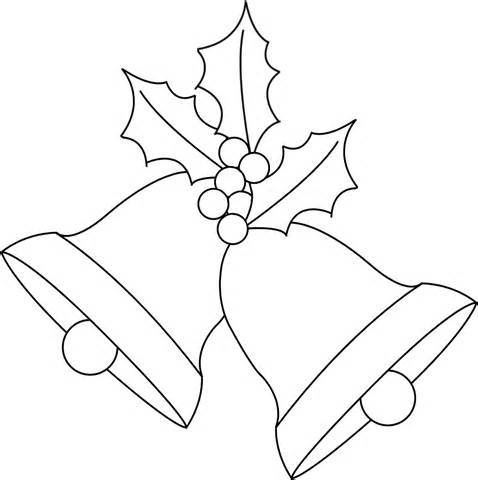
\includegraphics[width=1cm, scale=0.10]{bells.jpeg}
  AllSaints Rota 
%{\Huge Draft}
March -- April 2016
%  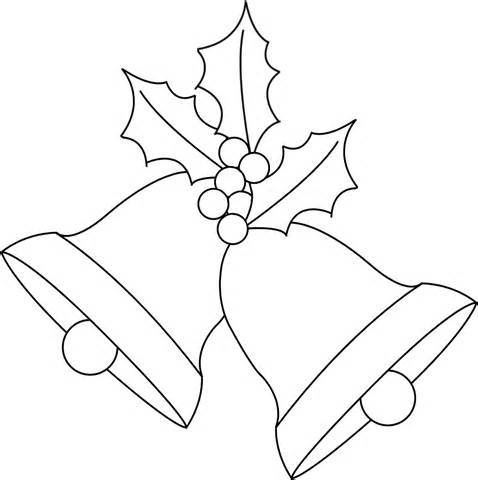
\includegraphics[width=1cm, scale=0.10]{bells.jpeg}
}%}
% \begin{figure}%[h]%t!]
%     \includegraphics{Koch-69a}
% \end{figure}
\vspace{0.5em}

% {\bf \Large \ldots for any final corrections - please check if dates are
%   impossible for you!} 
%\linebreak
%\rotatebox{90}{Advent}
%\begin{sloppypar}
{ \small
%% \begin{sidewaystable}[phbt]
% the 'P' column type is a ragged-right paragraph.  Uses array.sty
\newcolumntype{P}[1]{>{\raggedright}p{#1}}
\newcolumntype{X}[1]{>{\raggedright\arraybackslash}p{#1}}
\sloppy
\begin{tabular}{|%c | % Season
p{0.04\textwidth}| % Date
p{0.08\textwidth}| % Service
c| % Ldr
c| %Spkr
X{0.11\textwidth}| % Readings
X{0.07\textwidth}| % readers
p{0.05\textwidth}| % Prayers
X{0.08\textwidth}| %Side
% X{0.07\textwidth}| %Welc
X{0.09\textwidth}| % Tea
p{0.06\textwidth}| %Flwrs
p{0.05\textwidth}|}\hline %creche
%\begin{tabular}{|p{1.5cm}|p{1.8cm}|p{0.5cm}|p{0.5cm}|p{2.6cm}|p{2cm}|p{1.5cm}|p{2.4cm}|p{2.0cm}|p{2.2cm}
%\begin{tabular}{|p{1.6cm}|p{1.4cm}|p{0.6cm}|p{0.6cm}|p{2.8cm}|p{2cm}|p{1.5cm}|p{2.0cm}|p{2.0cm}|p{2.0cm}
%|p{1.8cm}|p{1.6cm}|}\hline
% heading
%{\bf
%& 
%\hline
 Date & Service & Leader & Spkr & Readings & Readers & Prayers &
Sidespersons & %Welcome Team &
 Tea &  Flowers & B'fast   \\ \hline % & Cr\^{e}che
\hline
6 Mar & 1st Sunday & \multicolumn{2}{c|}{DM} &   &  &  & Jim Donaldson   Richard Fieldhouse & L Hallatt R~Marshall J~Donaldson A~Walton & Linda Hallatt & Carol \& Richard \\ \hline
13 Mar & Holy Communion & DM & A C-P & Philippians 3:4b--14 John 12:1--8 & Ron Sherwin Mike Smithers & Shirley Hill & Peter \& Helen Tattersall &   B \& C Gleaves  G~Sly &   & Chris \& Brian \\ \hline
20 Mar & Morning Worship & DP & RM & Luke 19:28--40 & Ann Walton & Phil Marsh & Geoff Walton Jim Magnall &  A \& P McKenzie P Marsh &   & Robert \\ \hline
27 Mar & Easter Holy Communion & DM & DM & 1 Cor. 15:19--26 or Acts 10:34--43 John 20:1--18 or Luke 24:1--12  & Gillian Sly Alison McKenzie & Dot Phillips & Chris C-K Brian Gleaves  & P~\&~S~Gaskell E~Johnson & Pat Gaskell & Sue McFahn \\ \hline
3 Apr & Informal & CCK & CG & John 20:19--31 & Robert Marshall & Dot Graham & Jim Donaldson Pete McKenzie & B \& C Gleaves D~\&~R Graham   & Shirley Hill & Margaret \& Phil \\ \hline
10 Apr & Holy Communion & DM & DM & Revelation 5:11--14 John 21:1--19  & Brian Gleaves Richard Fieldhouse & Chris Gleaves & Chris C-K   Phil Marsh &   B \& V Bullock C~Fieldhouse  &   & Ann \& Geoff \\ \hline
17 Apr & Morning Worship & DM & DM & John 10:22--30  & Phil Marsh & Carol Fieldhouse & Richard Fieldhouse Tony Hallatt &  A \& P McKenzie R Marshall  &  & Pat \& Stephen \\ \hline
24 Apr & Holy Communion & DM & RM & Luke 13:31--35 &  Joy Kewney Tony Hallatt & Brian Gleaves & Geoff Walton Tony Hallatt & P \& S Gaskell G~Sly & Pat Gaskell & Chris C-K \\ \hline
1 May & 1st Sunday & \multicolumn{2}{c|}{DM} & Revelation 21:1--6 John 13:31--35 &   &  & Peter \& Helen Tattersall  & J Donaldson R~Marshall  E~Johnson P Marsh &   & Jacqui \\ \hline
\end{tabular}

\label{tab:LABEL}
%\end{table}\end{tabular}
%\end{sidewaystable}
}
%\end{sloppypar}

\vspace{1em}
%% Books: \begin{tabular}{|l|l|} \hline
% Gen & Genesis &
% Ex & Exodus \\
% Deut & Deuteronomy &
% Is & Isaiah \\
% Zep & Zephaniah &
% Zech & Zechariah \\
% 1 Cor & 1 Corinthians &
%Rom & Romans \\
  % Eph & Ephesians &
% 2 Cor & 2 Corinthians &
%Phil & Philippians &
%Col & Colossians &
%% 1 Thess & 1 Thessalonians 
%% \\
%% %&
%%   \hline
%% \end{tabular}
%\begin{tabular}{|c|c|c|c|c|c|c|c|c|c|c|}\hline
\begin{comment}
\begin{tabular}{|c|c|}\hline %|c|c|c|}\hline
{\bf People: } & \\
%AAWT & All-Age Worship Team & %DW & David Wightman &
%% MT & Marion Tugwood \\
%GVT & Gerri Tetzlaff \\
%LS & Lynne Spedding \\
BL & Barry Langman \\
%  GT & Graham Turner & RF & Richard Fieldhouse \\
%TH & Theresa Hayton & &  \\% JS & John Staley & 
%% IB & Ian Bishop &
%%  REM & Ruth Mock \\
%\\
%MS & Mike Strutt
%RW & Rob Wardle & & \\% & MH &  &  & \\
% VG & Vivien Gisby  & KR & Keith Ranger \\
% JG & Judith Gibson   &
% FH & Frances Hiles &
%& DM &  Dave Mock 
%AB & Andy Bull &
%KD & Kevin Dunn &
%PR & Philip Robinson &
%PS & Paul Spedding \\
% GT & Graham Turner &    %& JK & Joy Kewney   
%{\bf Abbreviations:}
%& nGP & No Godly Play 
%& tba & to be arranged \\
% {\bf Books: }  &  &   & 2 Cor & 2 Corinthians \\
%&   &  & 
%1 Thess & 1 Thessalonians & 
%\\ % & & & & & & & \\
%TG & Terry Gibson \\
% %FH & Frances Hiles & tba & to be arranged   \\ %\\ %JBu & John Buckley \\
% %BB & Barbara Bellfield & GC & Good Companions \\
% %  JM & John Mynett & MD & Mike Douglas \\
% % %  DW  & David Woodley & TG & Terry Gibson &%\\
% % %  RS & Ron Sutton & TS & Tony Sparham  \\
     \hline
\end{tabular}
\end{comment}
\end{center}
%\vspace{1em}
\begin{minipage}{0.65\textwidth}
%\begin{changebar} 
%{\bf 
{\footnotesize It would be helpful if sidespeople 
could arrive at 9.00am to ensure that service sheets and notice sheets are 
prepared and hymn numbers are put~up.
%}
%\end{changebar}
Please swap if you cannot do a date, see also list of names/tel nos.
Readers/Pray-ers -- if you swap, please let the service leader know.\\
I aim to update the master copy with changes as they
happen and make it available -- for those with internet access
 -- at
\url{http://www.capuchin.co.uk/AS-rotas.html} 
%\url{http://brock-marshall.no-ip.info/~robert/AS-rotas}
(Robert Marshall 262151)}
\end{minipage}
\hspace{1.5em}
\begin{minipage}{0.3\textwidth}
\ifpdf
%\begin{figure}%[hc]%t!]
%\hspace{2em}
\fbox{
%\hspace{2em}
%\includegraphics[bb=0 0 75 70]{team1} Macclesfield Team Parish
\vcenteredhbox{
\includegraphics[height=2.0cm, width=2.0cm]{newLogo}} Macclesfield Team Ministry
}
%\end{figure}
\else
\hspace{0.5em}
%\includegraphics[bb=0 0 75 70]{team1} Macclesfield Team Parish
\fi
\end{minipage}

\vspace{2em}
%Cr\^{e}che linked with 'Climbers' - contact Margaret Marsh
{\footnotesize 
%% Corrections to \url{&#109;&#97;&#105;&#108;&#116;&#111;&#58;&#114;&#111;&#98;&#101;&#114;&#116;&#64;&#99;&#97;&#112;&#117;&#99;&#104;&#105;&#110;&#46;&#99;&#111;&#46;&#117;&#107;}
%% \begin{htmlonly}
%% For corrections you can email me on the link at the foot of
%% \url{http://www.chezmarshall.freeserve.co.uk} (Robert Marshall)
%% a pdf form of the rota is available at
%% \url{http://brock-marshall.no-ip.info/~robert/AS-rotas/} - when my
%% home machine is booted!!

%% The reading listings are available at
%% \url{http://www.cofe.anglican.org/worship/liturgy/commonworship/resources/downloads/csvfile.html}
%% %http://www.cofe.anglican.org/commonworship/lect/lectfront1.html}.
%% Text of the readings can be found at
%% \url{http://divinity.library.vanderbilt.edu/lectionary/} - we are in Year B
%%  but the readings sometimes differ from the Anglican version!

%% %{\tiny  \$Id: AllSaintsRota.tex,v 1.62 2011/03/05 08:34:43 robert Exp $    }
%% %  \date{Revision \RCSRevision, \RCSDate}
%% %}

%% \end{htmlonly}
  \RCS$Revision: 1.62 $ % or any RCS keyword
  \RCS$Date: 2011/03/05 08:34:43 $

%{  \ $Id: AllSaintsRota.tex,v 1.62 2011/03/05 08:34:43 robert Exp $    }

%\begingroup
%\ifpdf
%\end{landscape}
%\fi
%\endgroup
}
\end{document}


